\section{R1}
Just like every projects, the first steps consisted in understanding the problematic, the scope and the challenges. We made a few researches regarding road quality assessment and related topics in order to learn about already existing solutions or relevant methods.\\

We were then able to define sprint objectives and organise them by using \textit{user stories} and \textit{sprint complexity} (Figure \ref{user_stories}). The sprints were then used to plan the project progress.

\begin{figure}
    \center
    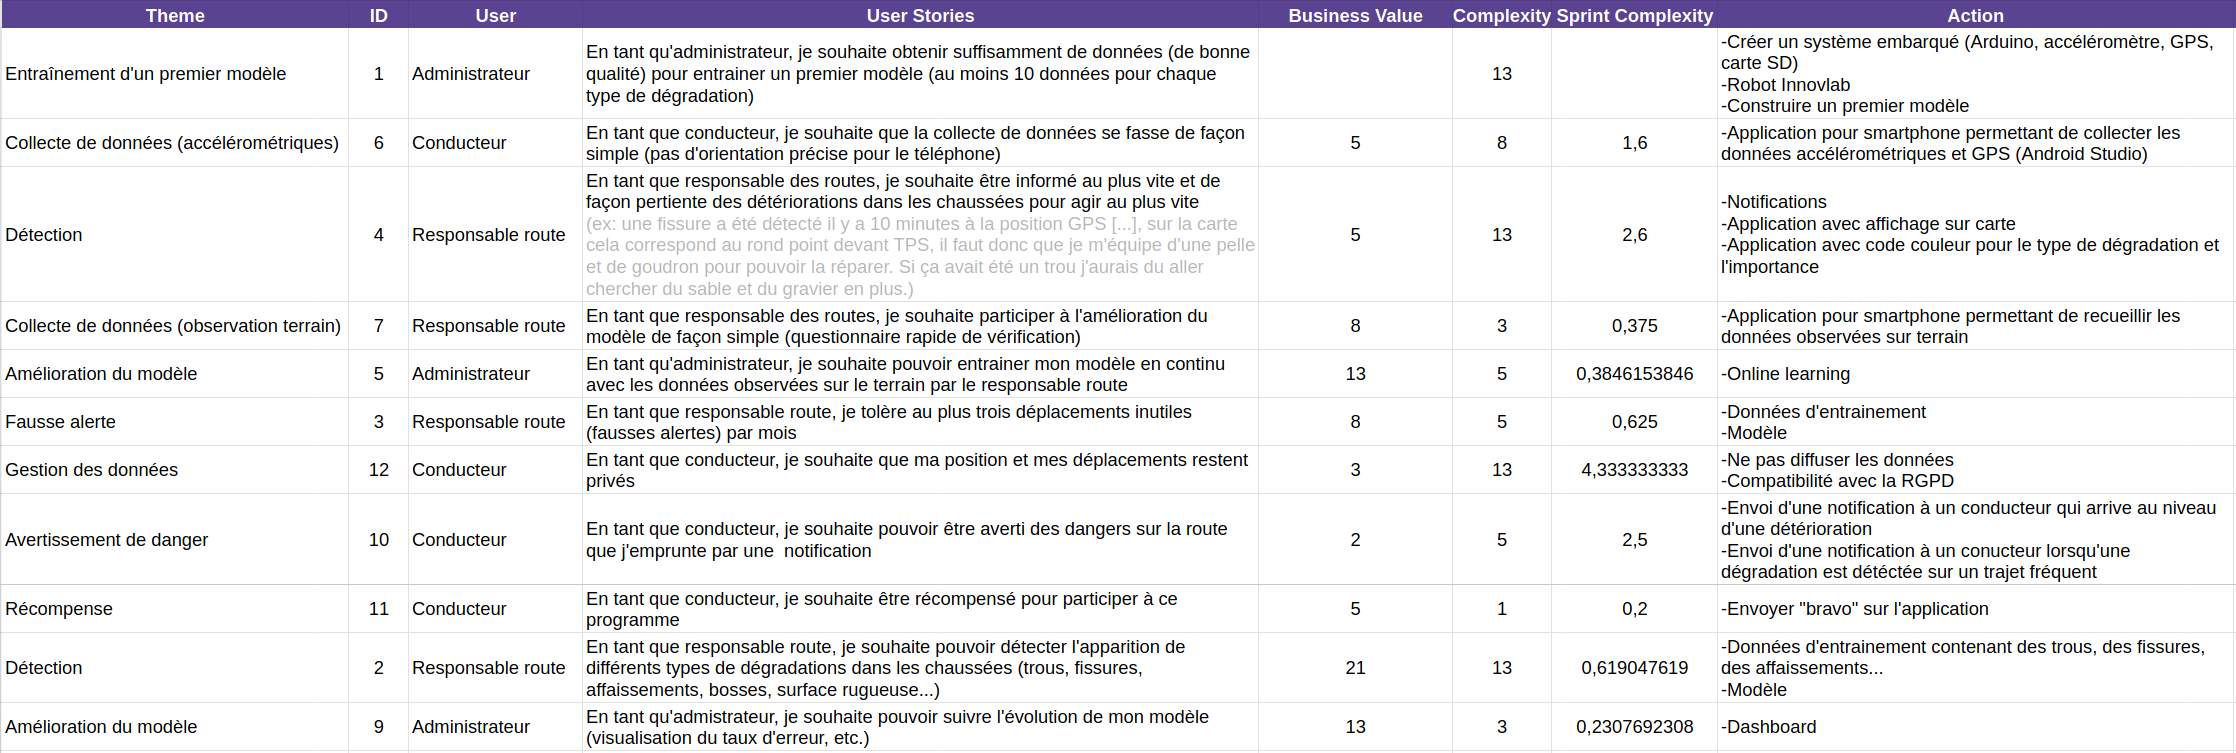
\includegraphics[scale=.2]{img/user_stories.png}
    \caption{User Stories}
    \label{user_stories}
\end{figure}

The project was devided in three distinct parts:
\begin{itemize}
\item Collect data
\item Train an AI
\item Develop an application
\end{itemize}
For the most part, these three aspects of the project can be developped independantly meaning we will be able to divide tasks in the future.\\

\begin{figure}
    \center
    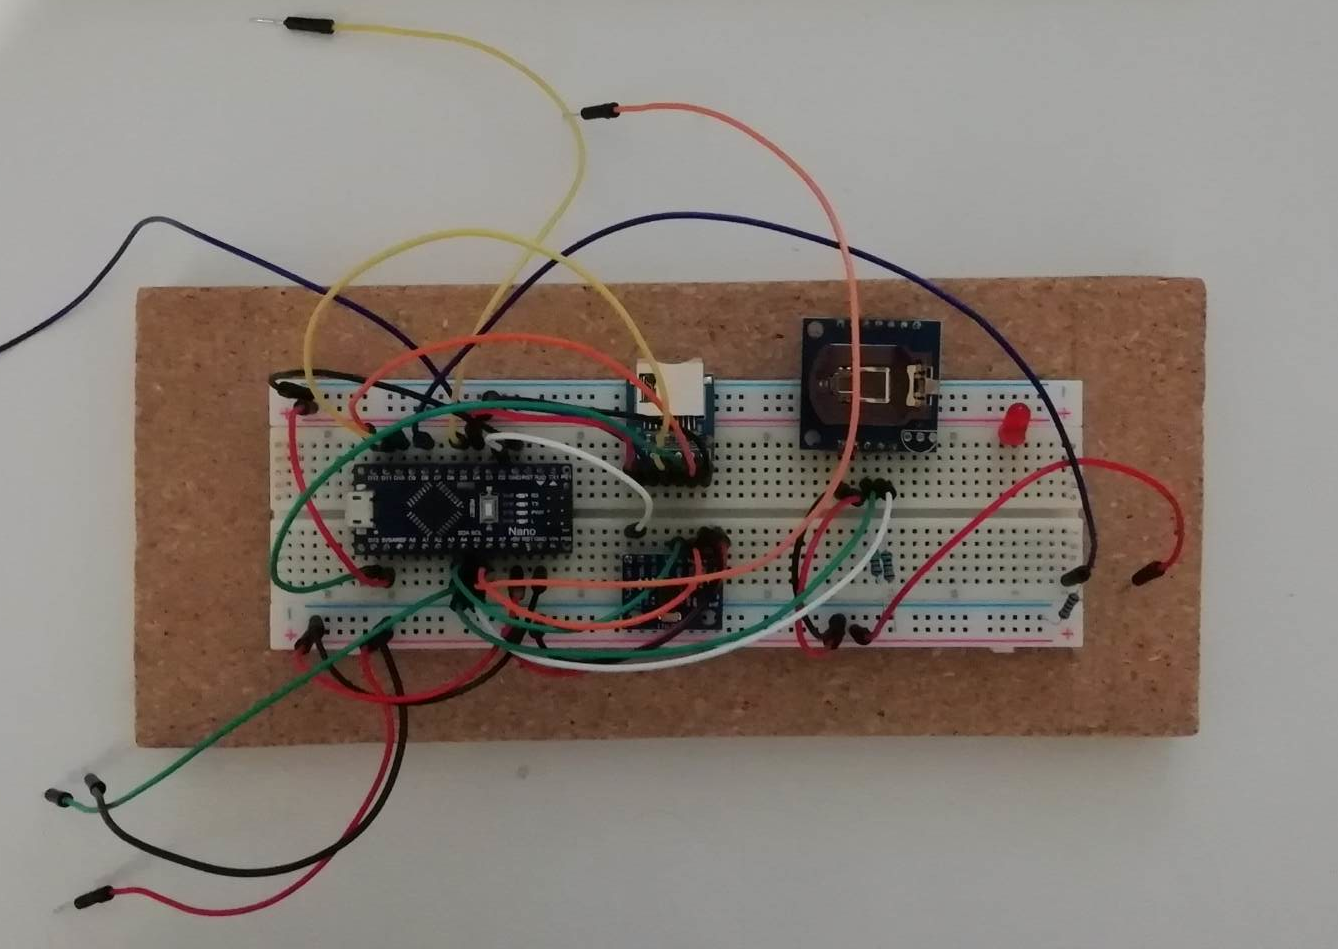
\includegraphics[scale=.8]{img/breadboard.png}
    \caption{Prototype of the Arduino device}
    \label{bread}
\end{figure}

However, as the entiere project is based on acceleration data, we decided to focus on data collection at the beginning. We thought it would help us understanding the project furthermore (what kind of data we are working with, how to collect acceleration data, what does it look like...) and avoid any misleading assumption and useless work.\\
We designed a basic device around an Arduino Nano and an IMU that would provide us sample of acceleration data to visualise and analyse. At the time of the last review the device was still in developement (Figure \ref{bread}) due to unexpected behavior of the Arduino controler when connecting multiple modules on the I²C bus.